\chapter{Mechanical Design}
\label{chap:7}
In this section brief description of VSCMG test-bed mechanical design is described. Various manufacturing techniques has been employed and design choices are made in order to make sure simplicity and keeping overall cost within affordable range. 
\section{System Overview}
\newacronym{sgcmg}{SGCMG}{Single Gimble Control Moment Gyroscope}
Test bed is designed in order to simulate attitude control system of satellite equipped with momentum exchange device. A re-configurable and modular designed is realised so that various arrangements of Reaction Wheel, CMG configurations could be tested with minimum modification. Primary design consist of four \acrshort{sgcmg} units arranged in pyramid configuration on sandwich of two acrylic sheets as main platform to hold entire electronics and power system. This platform is balanced on sharp pin keeping center of gravity of entire unit below but close to pin point. This pin joint allows complete 360 degree of rotation around yaw axis as well as $\pm 60 \deg$ in roll and pitch axis constraining translation motion. Selected degree of freedom is sufficient for most of the GNC verification requirements. Entire assembly is balanced on tip placed on a small custom made tripod, a rendered view of test bed is shown in \ref{fig:my_AssemblyACR}

\begin{figure}[ht]
    \centering
    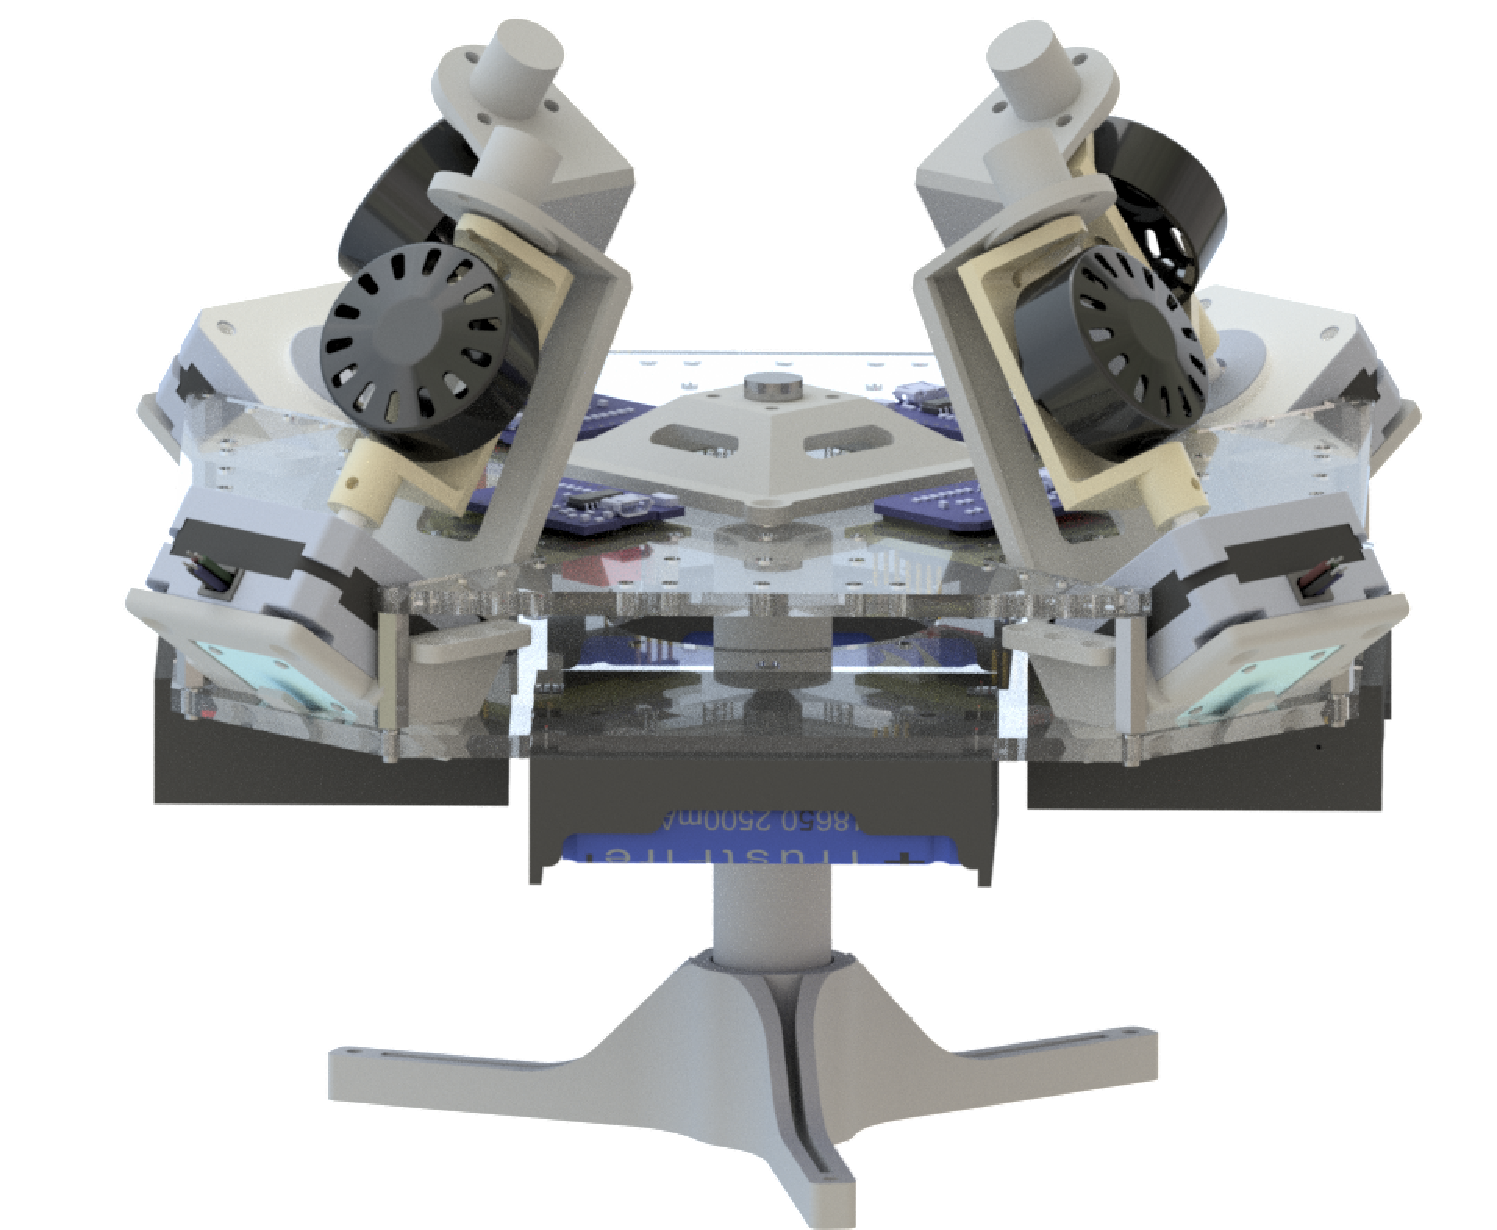
\includegraphics[width=0.55\textwidth]{figures/Assembly/AssemblyACR - Transperent.pdf}
    \caption{VSCMG Attitude Control System test bed Assembly (Rendered)}
    \label{fig:my_AssemblyACR}
\end{figure}

\section{Reaction Wheel Motor}
\newacronym{bldc}{BLDC}{Brushless DC}
Three phase permanent magnet \acrfull{bldc} outrunner motor is selected for reaction wheel. As name suggest brushless motor does not have brush contact for electric power and needs special commutation sequence in order to properly operate at desired torque and speed explained in next chapter. These are highly efficient and provide greater torques compared to brushed dc motors \cite{bldc}. Outrunner motor has external rotor casing with attached permanent magnets and inner stator with three phase coil winding. Very low cost high RPM and High rotor inertia \acrshort{bldc} motors found shown in \autoref{fig:BLDC2} which can rotate at 900 RPM/Volt and has with inertia $3.140 kg \ mm^2$ evaluated using CAD software. This configuration is suitable for ACS testbench requirements.
\begin{figure}[ht]
    \centering
    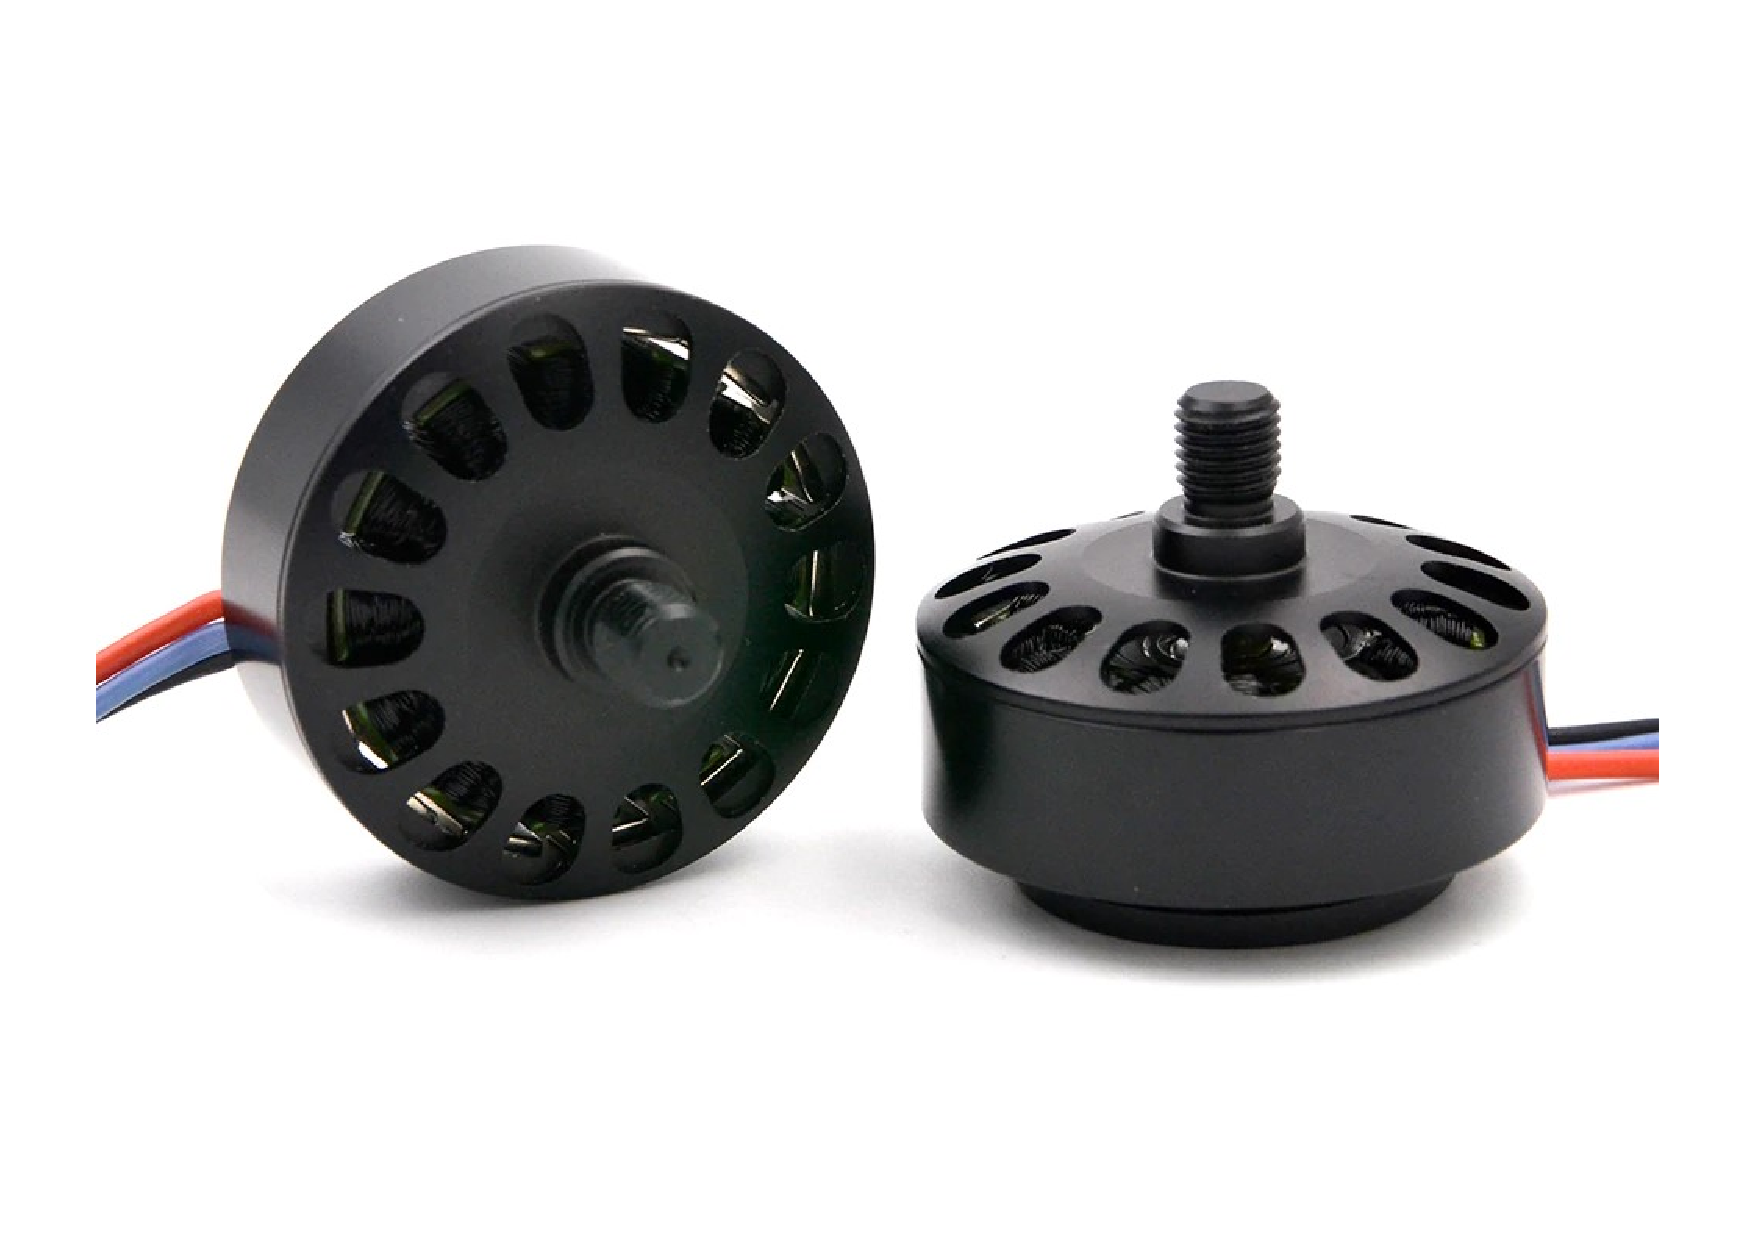
\includegraphics[width=0.80\textwidth]{figures/Assembly/BLDC2.pdf}
    \caption{Three phase, outrunner, Brushless DC Motor as reaction wheel}
    \label{fig:BLDC2}
\end{figure}

\section{Gimbal Motor}
From numerical simulations performed in earlier chapters it is noted that gimbal motor speed is relatively very slow hence 4 wire stepper motor is selected as gimbal actuator. As shown \autoref{fig:NEMA17} in Standard NEMA 17HS081004 motor of 20mm length with $1.8 \deg$ step angle \cite{web:ds_nema17} is used due to simplicity of control by using appropriate step sequence and and ability of micro stepping in order to have precise resolution. These type of motors are available in standard form factor and in affordable cost since most of the 3d printers available in market are equipped with such motor. 
\begin{figure}[ht]
    \centering
    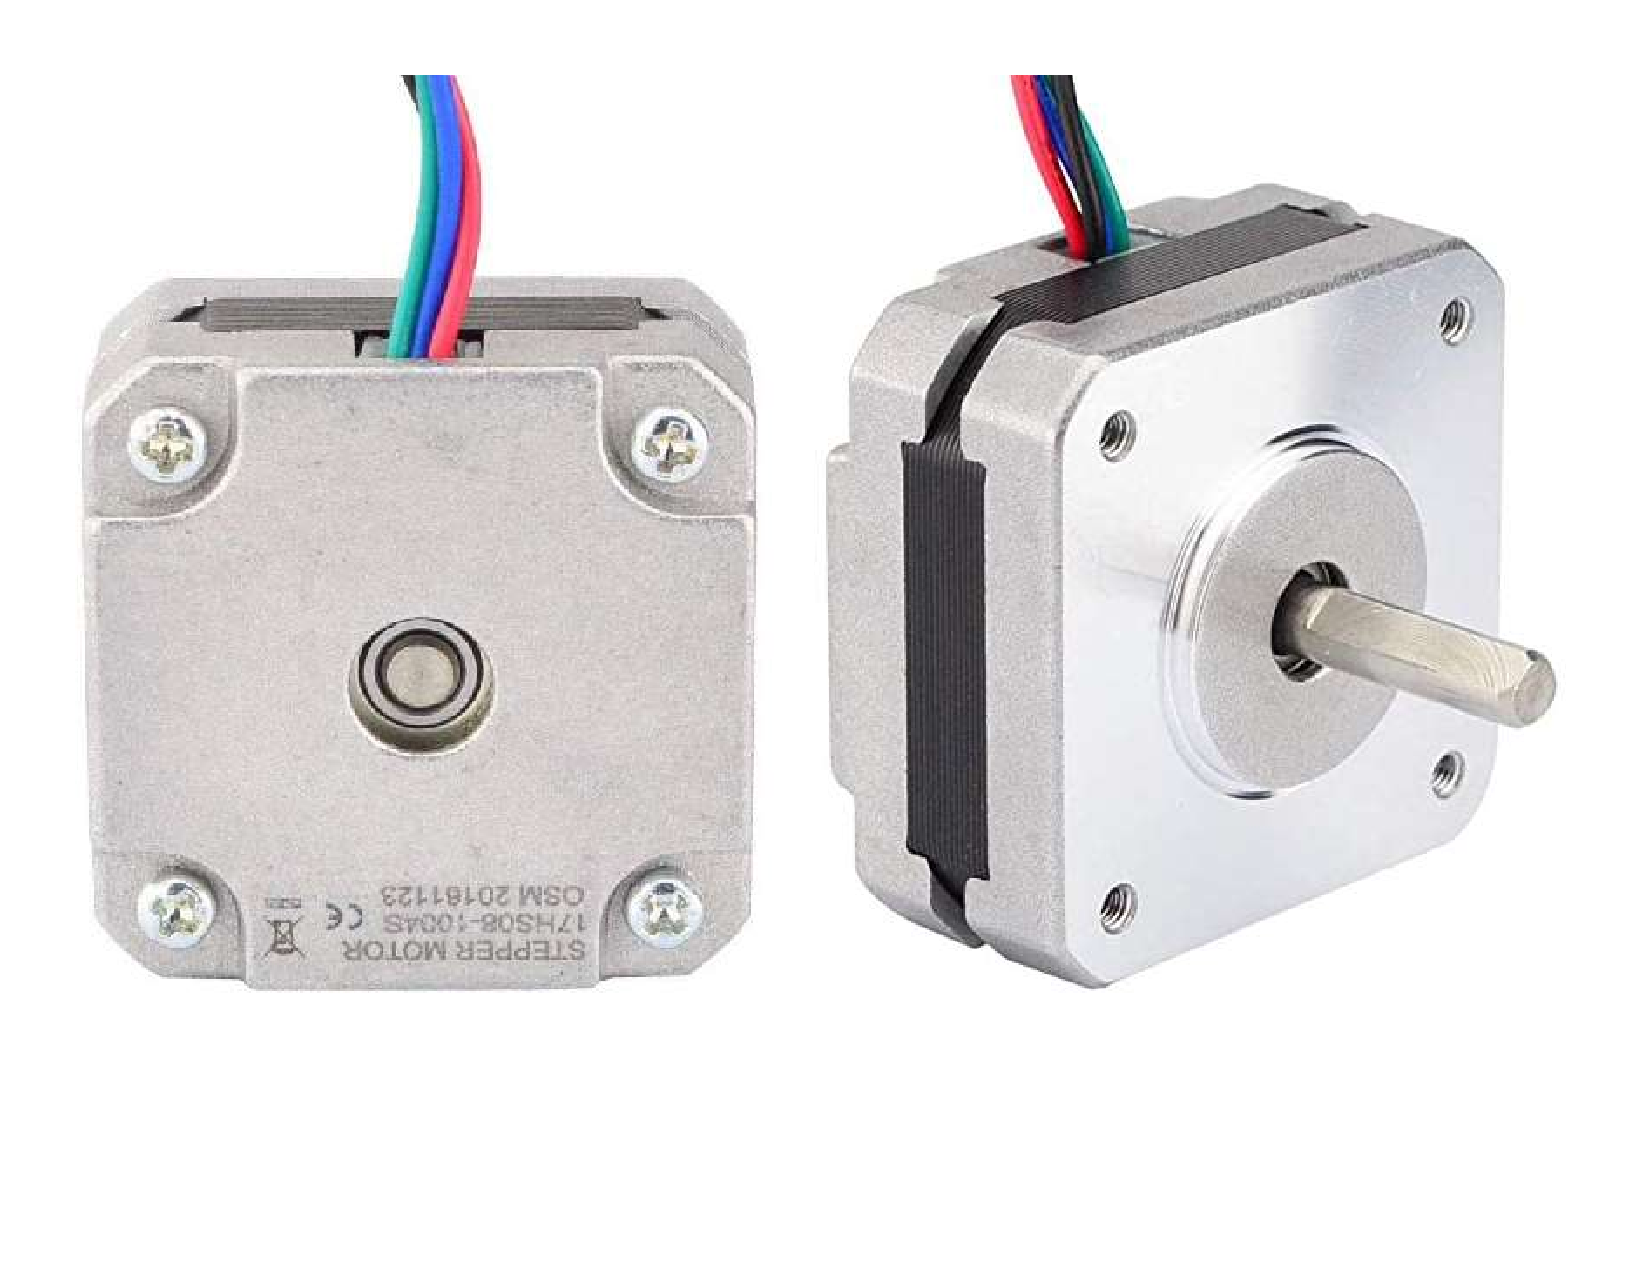
\includegraphics[width=0.80\textwidth]{figures/Assembly/NEMA17.pdf}
    \caption{NEMA 17HS081004 Stepper motor \cite{web:ds_nema17}}
    \label{fig:NEMA17}
\end{figure}
\section{Slip Ring}
In order to transfer power from stationary component to rotating component slip ring is used. 6 channel slip ring is used as shown in \autoref{fig:SLP_RNG} it has 6 wires going in to large stationary part with flange and coming out from rotating end. Selected slip ring has 1A nominal current carrying capacity at maximum 300 RPM. One of the most important component needs to taken care of while designing SGCMG assembly.

\begin{figure}[ht]
    \centering
    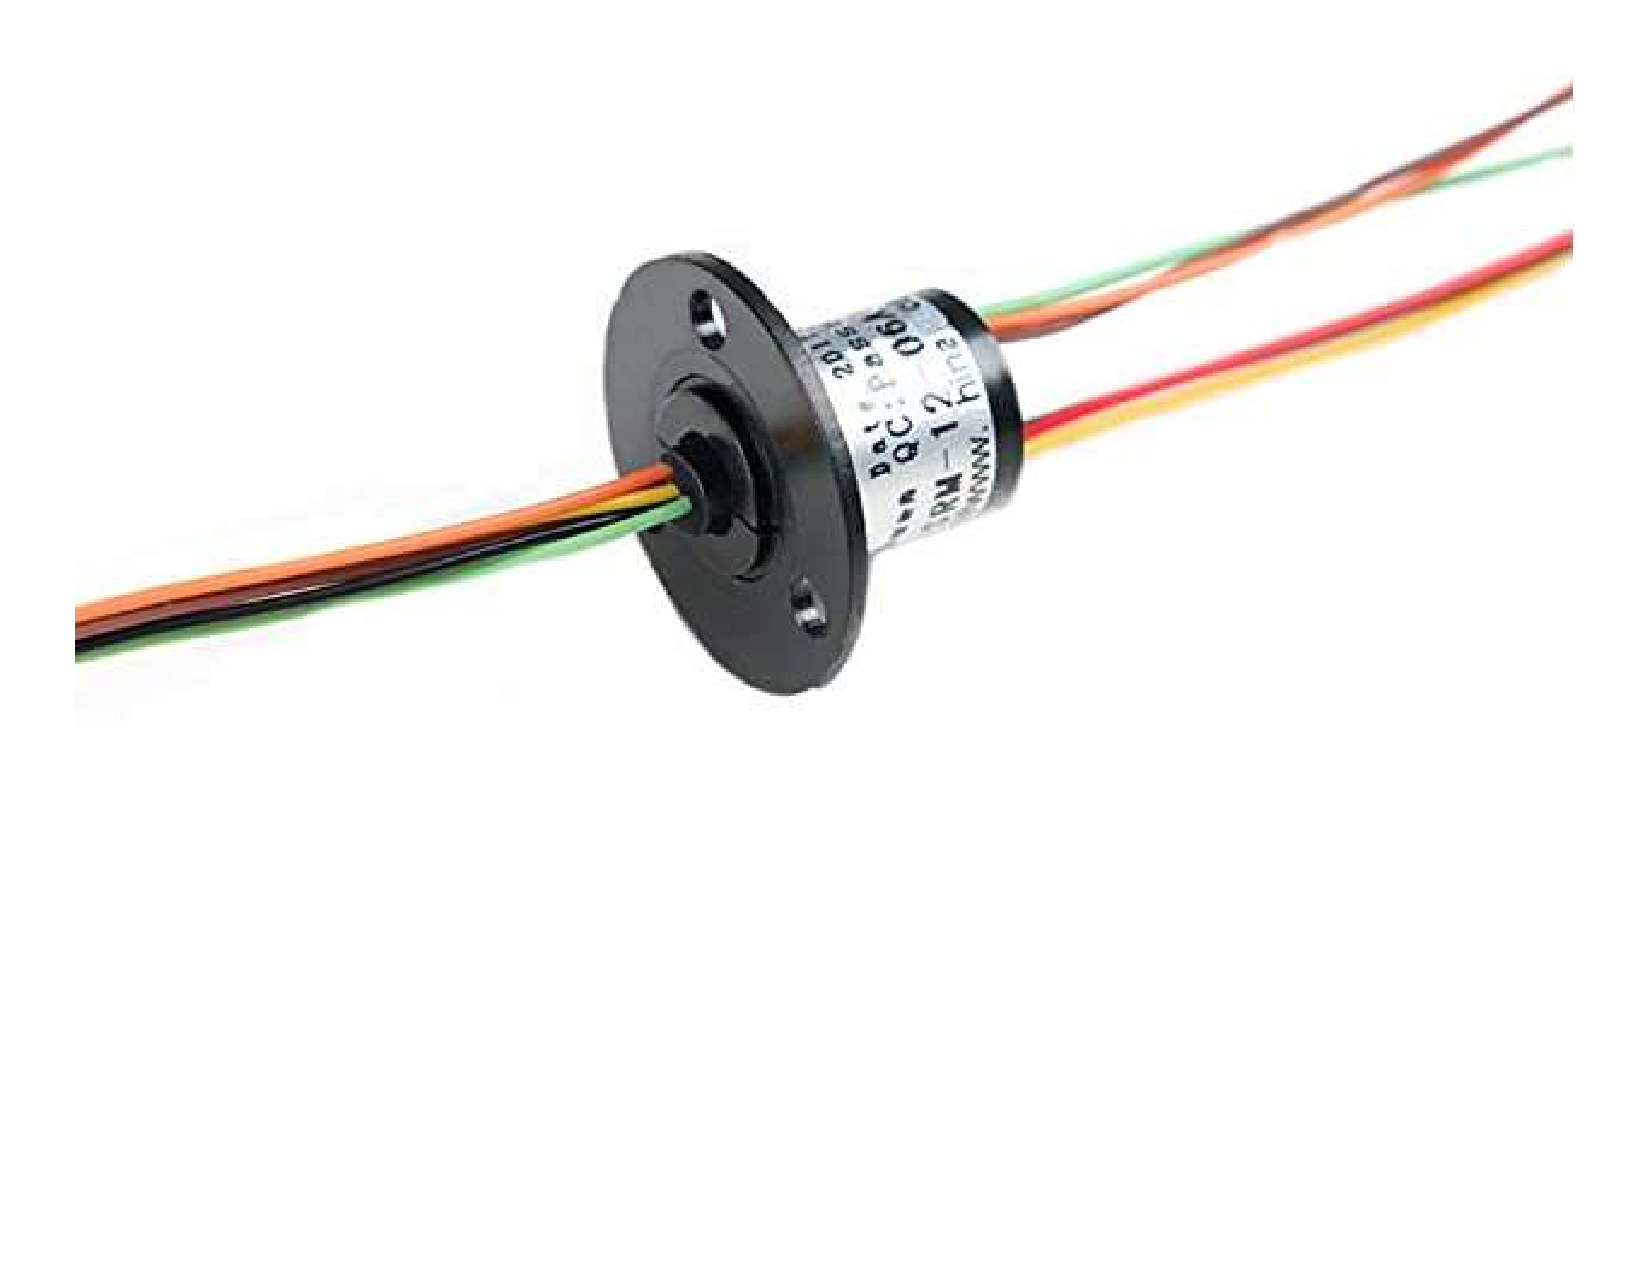
\includegraphics[width=0.60\textwidth]{figures/Assembly/SLP_RNG.pdf}
    \caption{6 channel Slip Ring}
    \label{fig:SLP_RNG}
\end{figure}


\section{SGCMG Assembly Design}
In order to achieve modular design, an unit of \acrlong{sgcmg} sub assembly is designed. Each SGCMG unit has a reaction wheel motor mounted on a gimbal attached to gimbal motor keeping reaction wheels center of mass in line with gimbal rotation axis. Since gimbal motor may perform multiple revolutions, inner motor which is reaction wheel needs to be powered such a way that power cables should not hinder and entangle due to rotations of outer gimbal motor. For this reason a power wires for reaction wheel motors are passed through slip ring which allows transmission of power supply from stationary to rotating structure. A magnetic encoder is placed behind the gimbal motor in order to have angle and angular velocity feedback from gimbal motor, an SGCMG unit is shown in. Two structural components of \acrshort{sgcmg} fabricated with 3D printing ABS material are:
\begin{itemize}
    \item Gimbal Motor Mount
    \item Reaction Wheel Mount
\end{itemize}
\subsection{Gimbal Motor Mount}
Important structural component of SGCMG is designed to support stepper motor at one end and slip ring at other end. Special attention given so that Reaction wheel mount which would be attached to gimbal motor shaft should have enough clearance to allow free rotation of Reaction Wheel Mount. Power to the reaction wheel is provided through slip ring, hence a provision is made to hold slip ring with it's axis in line with gimbal motor shaft as shown in \autoref{fig:GMBL_MNT}. A slot at the end of mount allows proper placement of magnetic encoder in order to have feedback from stepper motor. A complete standalone SGCMG unit is shown in \autoref{fig:SGCMG_ASM}.

\begin{figure}[ht]
    \centering
    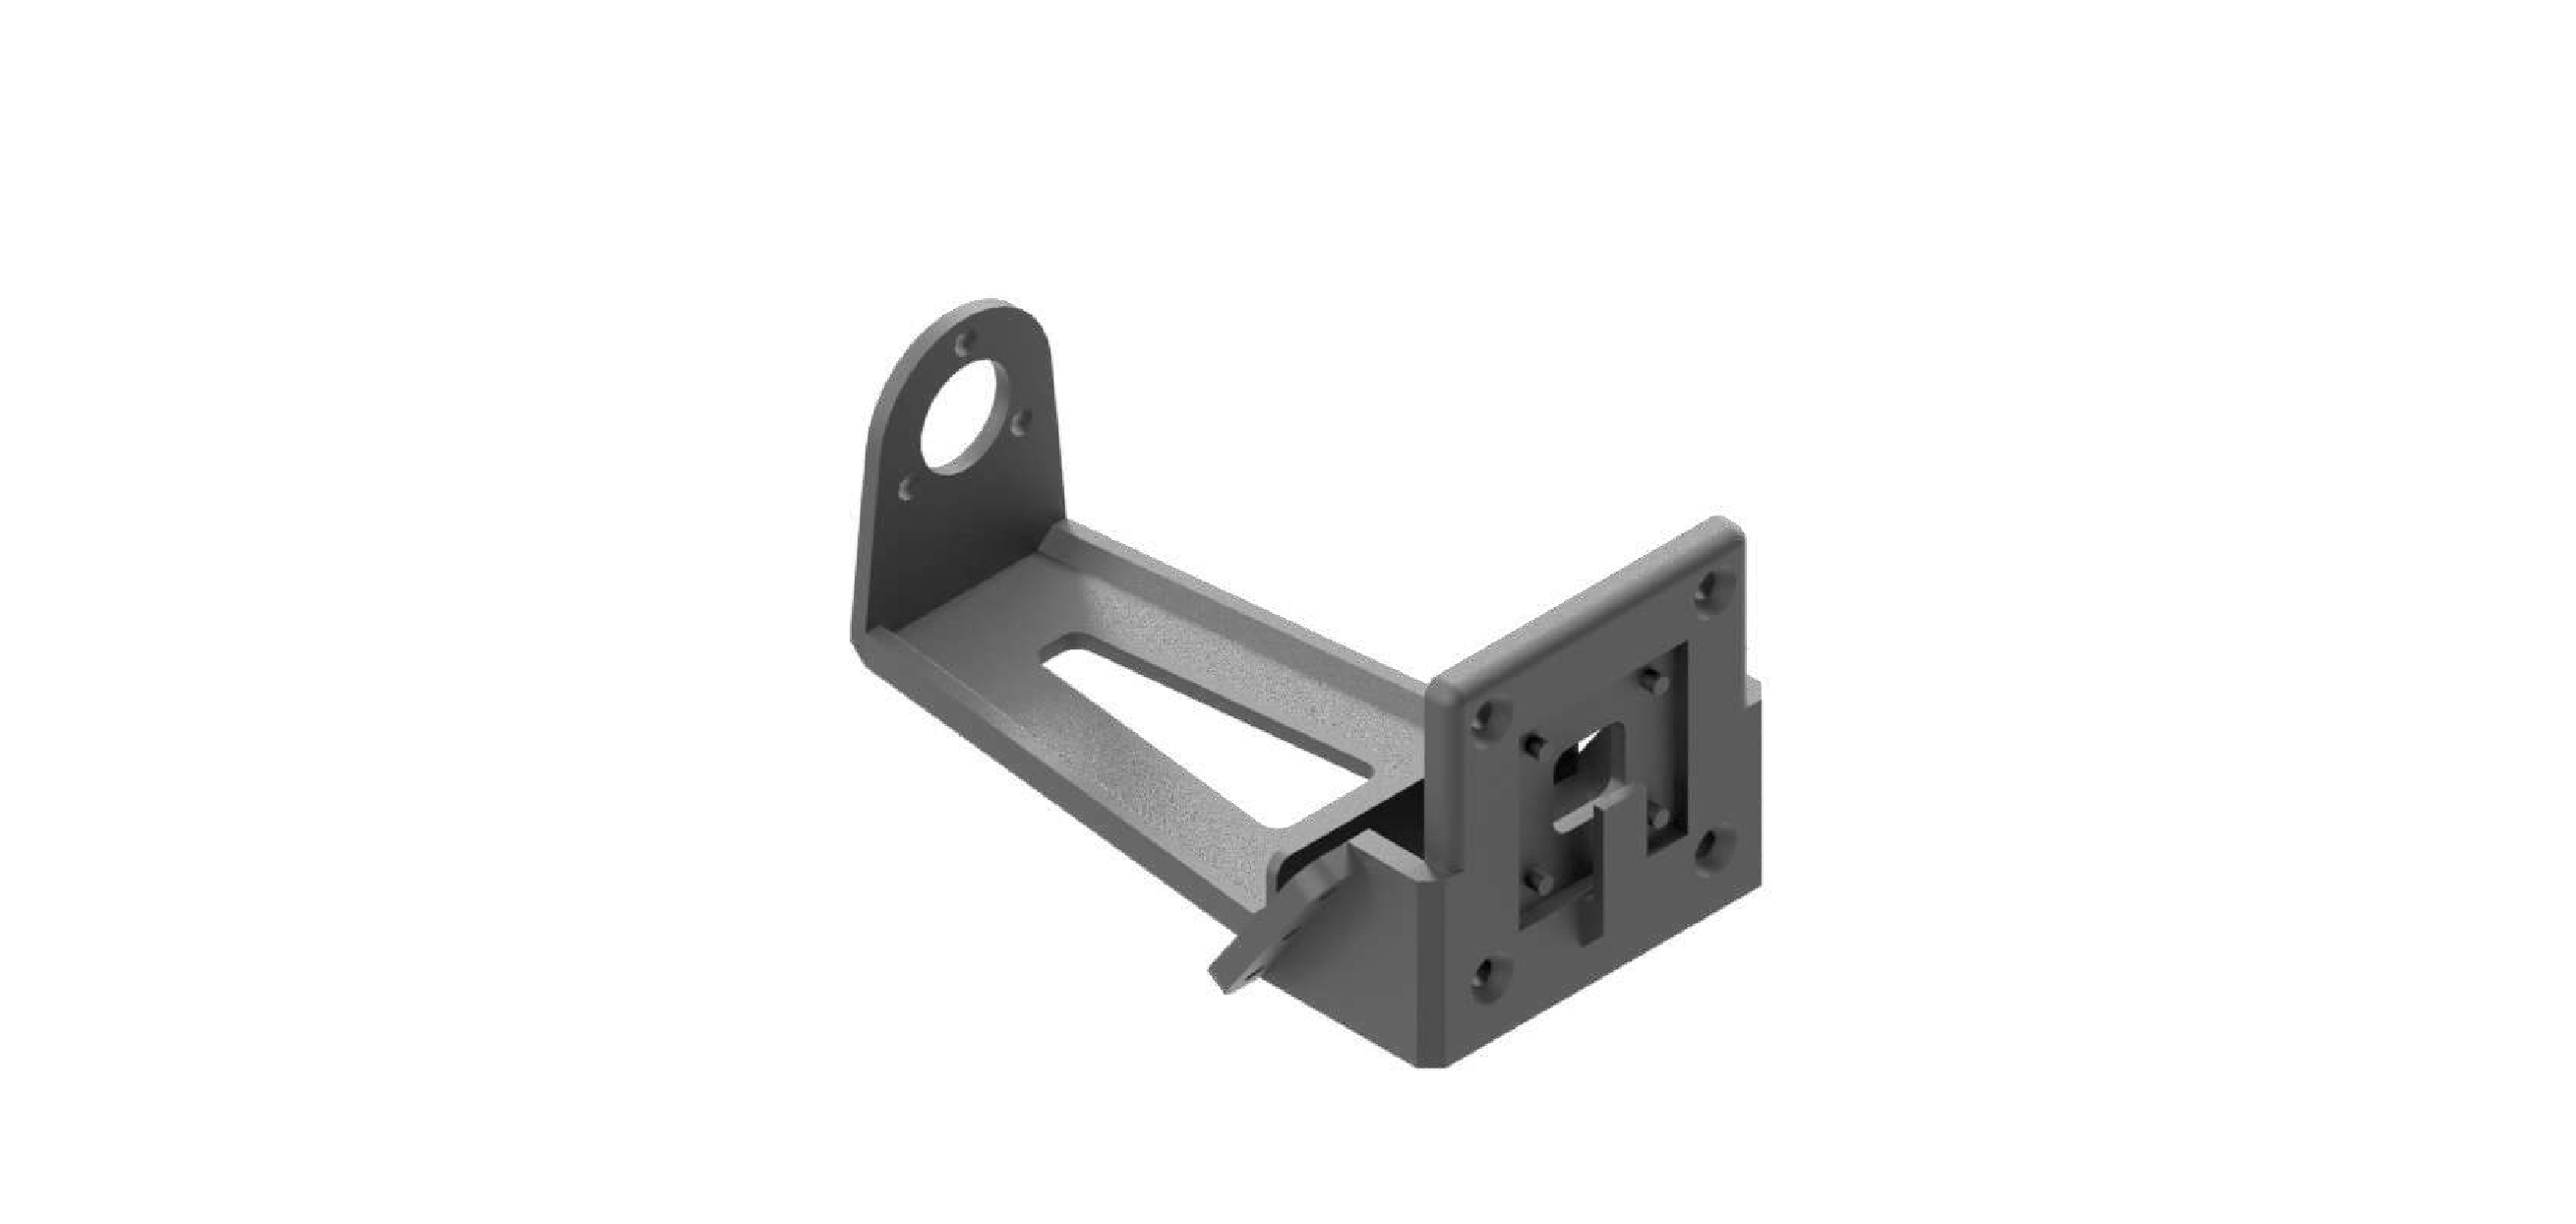
\includegraphics[width=\textwidth]{figures/Assembly/STP_MOUNT.pdf}
    \caption{Gimbal Motor Mount (Rendered)}
    \label{fig:GMBL_MNT}
\end{figure}

\subsection{Reaction Wheel Mount}
C shaped mount is used to hold Reaction Wheel motor as shown in, BLDC motor is mounted on web of C channel. Reaction wheel mount is connected to stepper motor shaft at one end while other end is supported by rotating end of slip ring. Special attention is paid in order to connect \acrshort{bldc} wires from slip ring without hindering any component. 

\begin{figure}[ht]
    \centering
    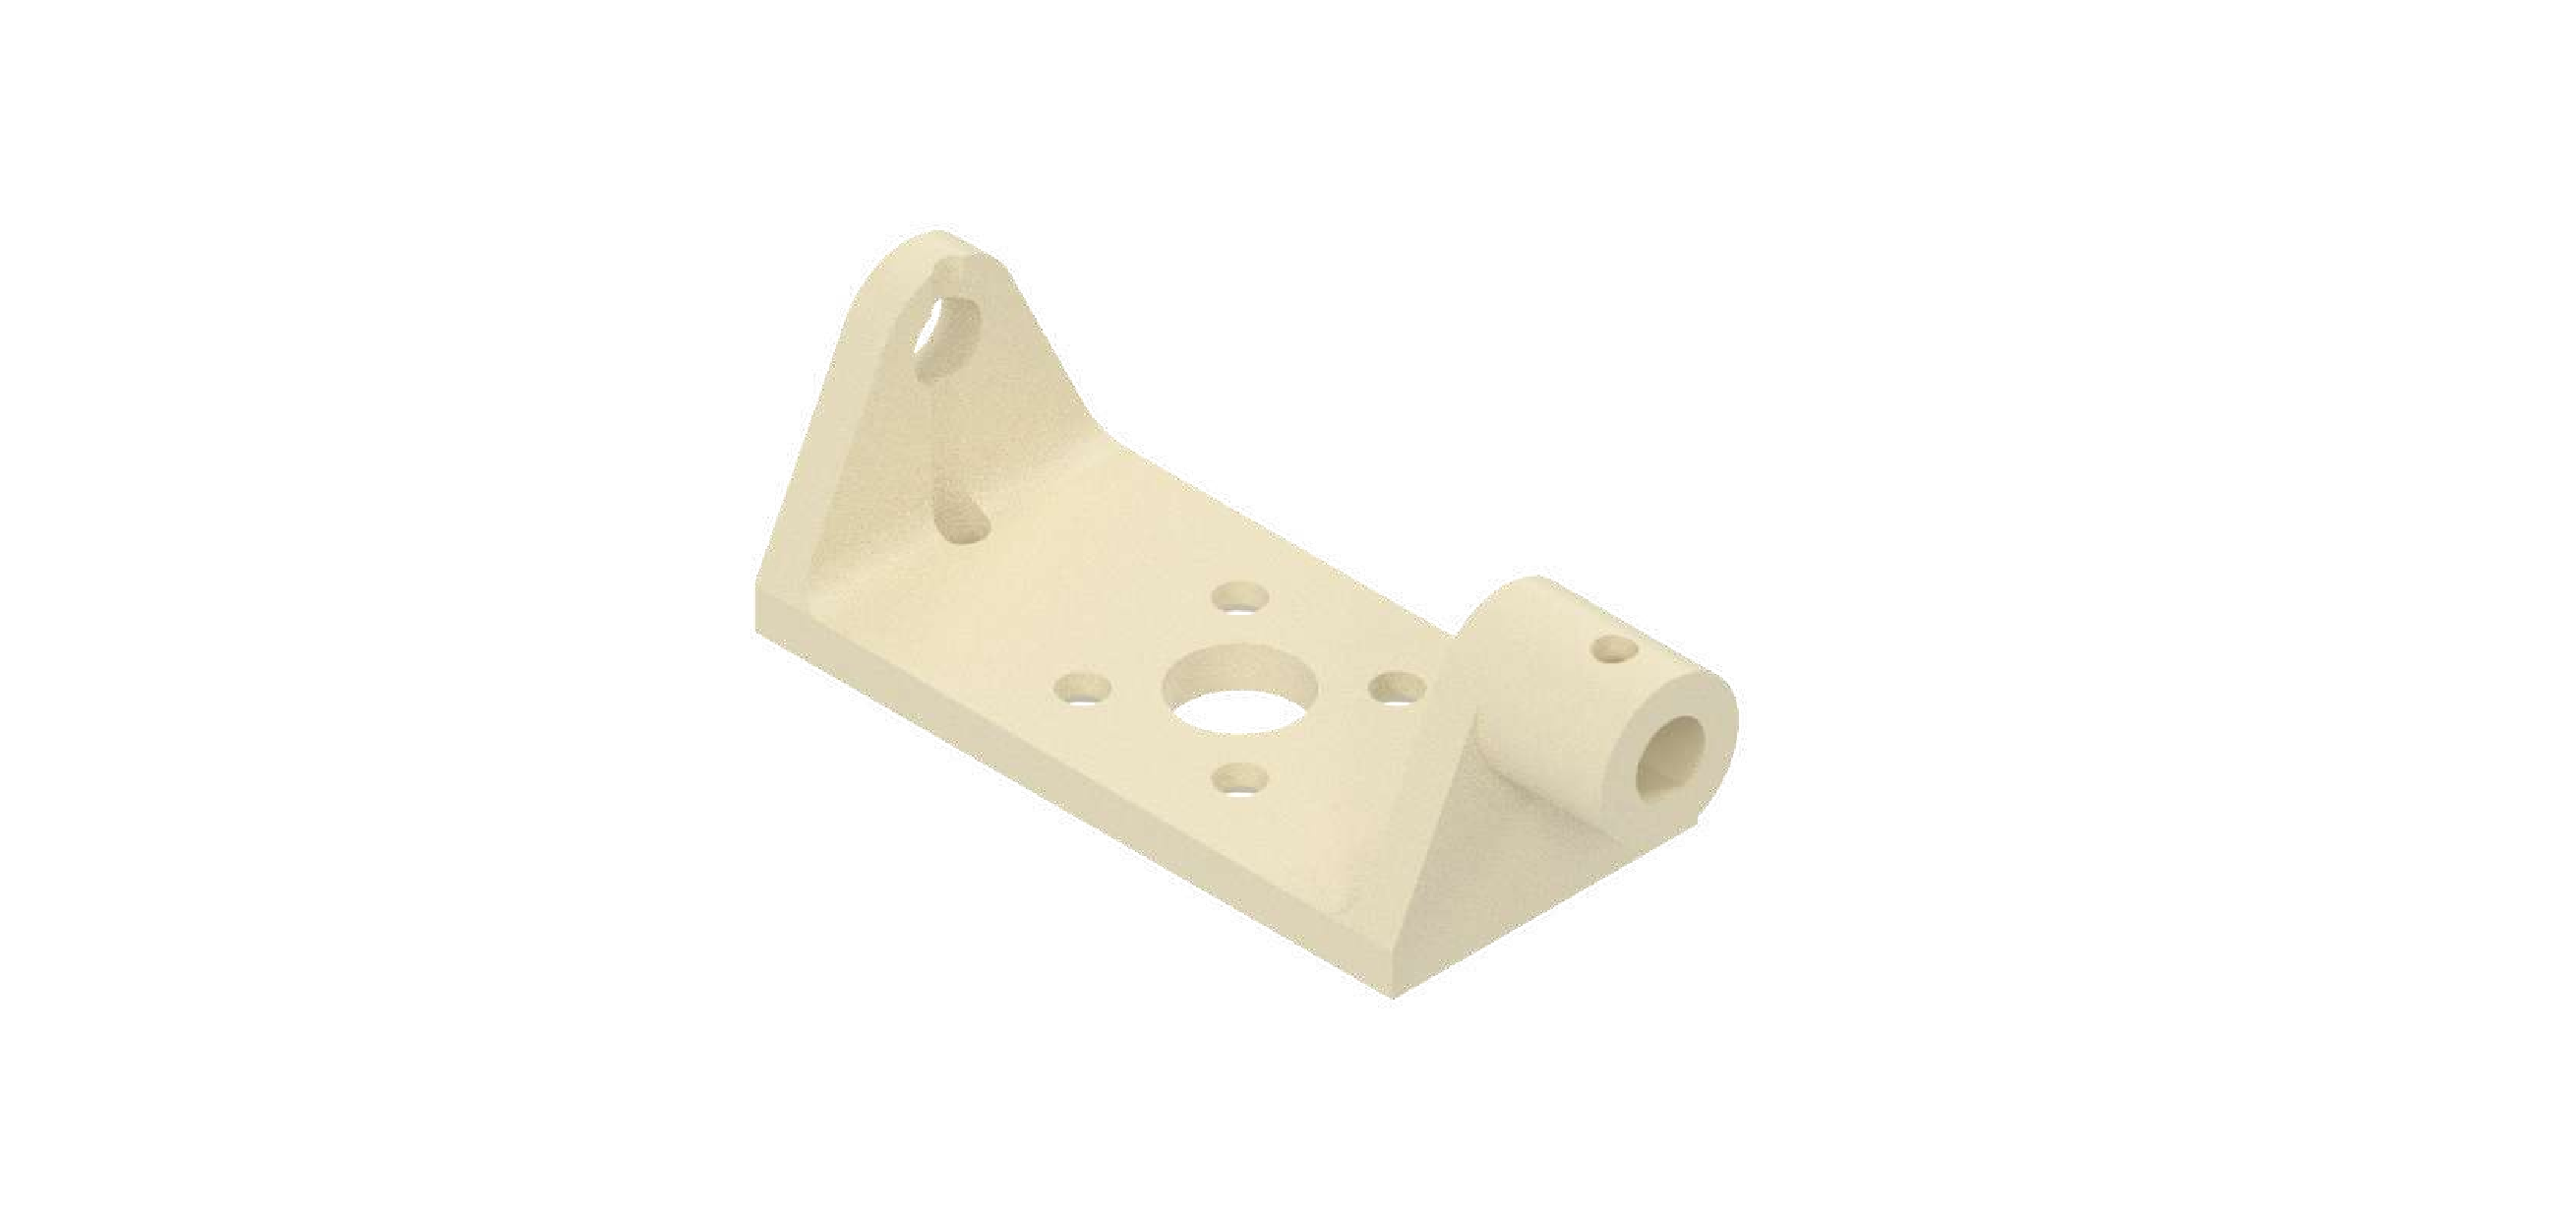
\includegraphics[width=\textwidth]{figures/Assembly/rwMount.pdf}
    \caption{Reaction Wheel Motor Mount (Rendered)}
    \label{fig:RW_MNT}
\end{figure}

\begin{figure}[ht]
    \centering
    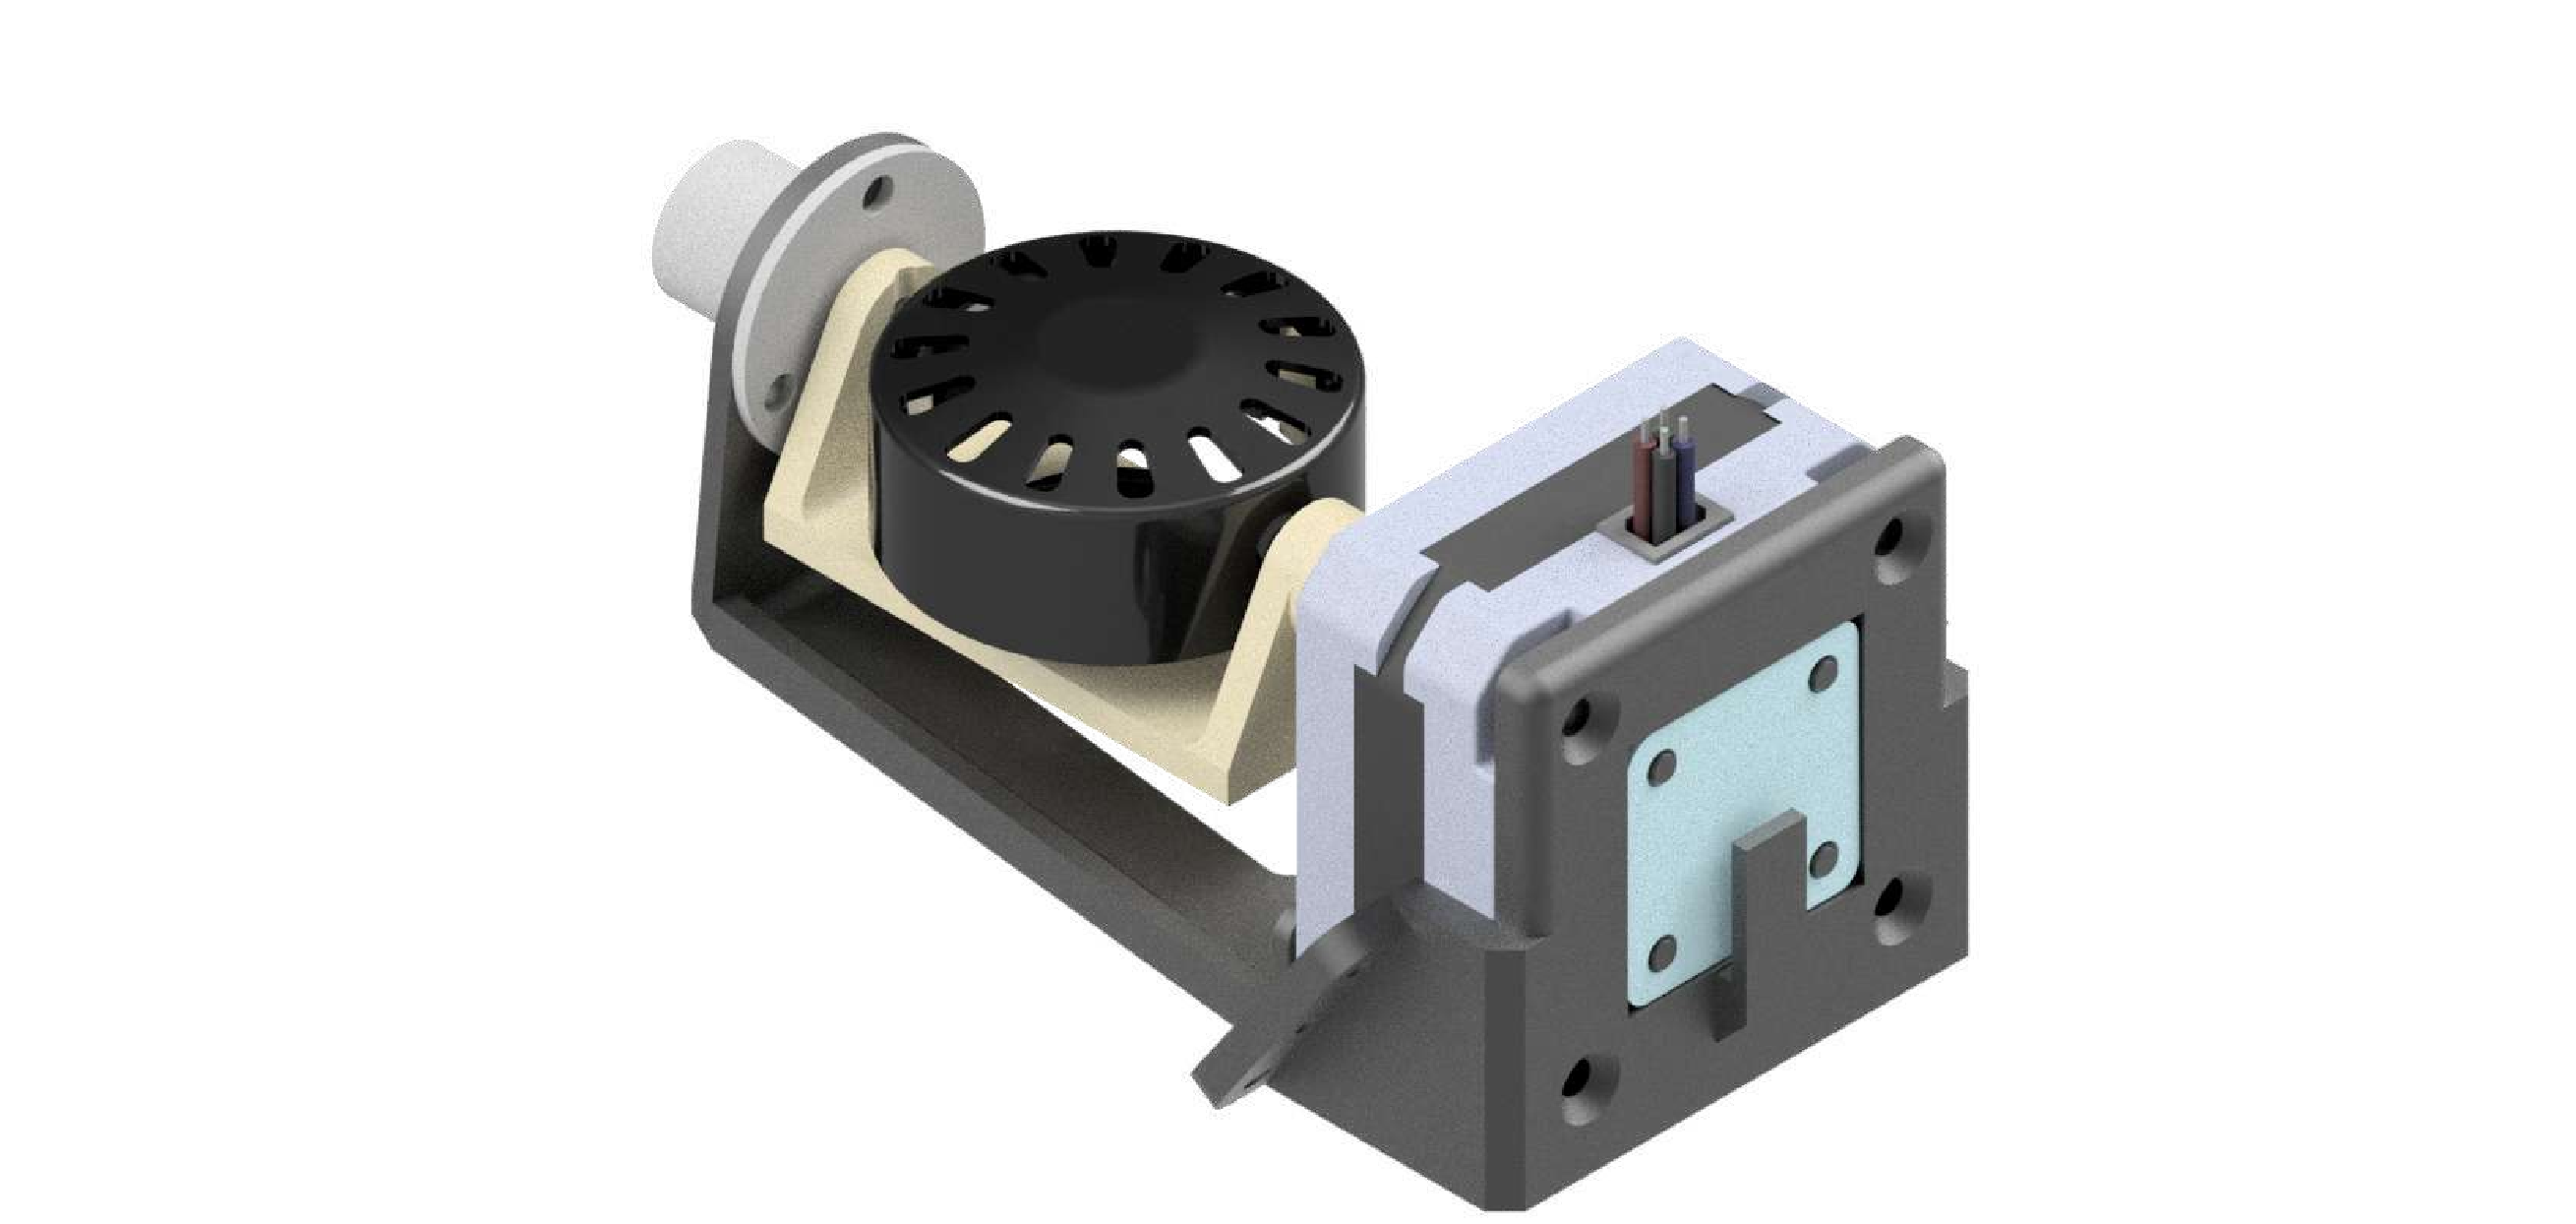
\includegraphics[width=\textwidth]{figures/Assembly/SGCMG.pdf}
    \caption{Complete SGCMG assembly (Rendered)}
    \label{fig:SGCMG_ASM}
\end{figure}

\section{Base Platform}
Central structure of test bed which shall hold together all the SGCMG units, power system and other required electronics components. Base platform consist of two acrylic plates fabricated using laser cutting as per design, sand-witched together using spacers. This type of two layer design incorporated so that most of the electronic components and PCBs can use the place between two plates. Batteries are fixed on bottom plate whereas four SGCMG units are bolted on top plate in order to bring center of mass as close to plates as possible. Entire design is kept symmetric in order to simplify manufacturing but most important mass balancing requirement. Most important requirements is the entire platform needs to be balanced on sharp tip with it's center of mass below but closer to tip. Since there will be uncertainties in mass distribution due to the fact presence of wiring and other non modeled components we can not guaranty that CoM is at desired location. Hence a threaded Allen bolt with sharp tip is used. A 3D printed pyramid structure is mounted on top base plate. This part has threaded hole at the center in order to hold sharp cone pointed bolt. This sub assembly shown in \autoref{fig:PLATFORM_TIP_ASM} allows variable position of pivot so that distance of center of mass from pivot along z axis can be shifted as per requirement. A small 3D printed tripod is designed on which entire base platform shall be balanced. Due to the fact that sharp tip may easily damage 3D printed structure, a steal coin is fixed on the top of tripod shaft and entire satellite platform will rest on this steel coin at the edge of tip.

\begin{figure}[ht]
    \centering
    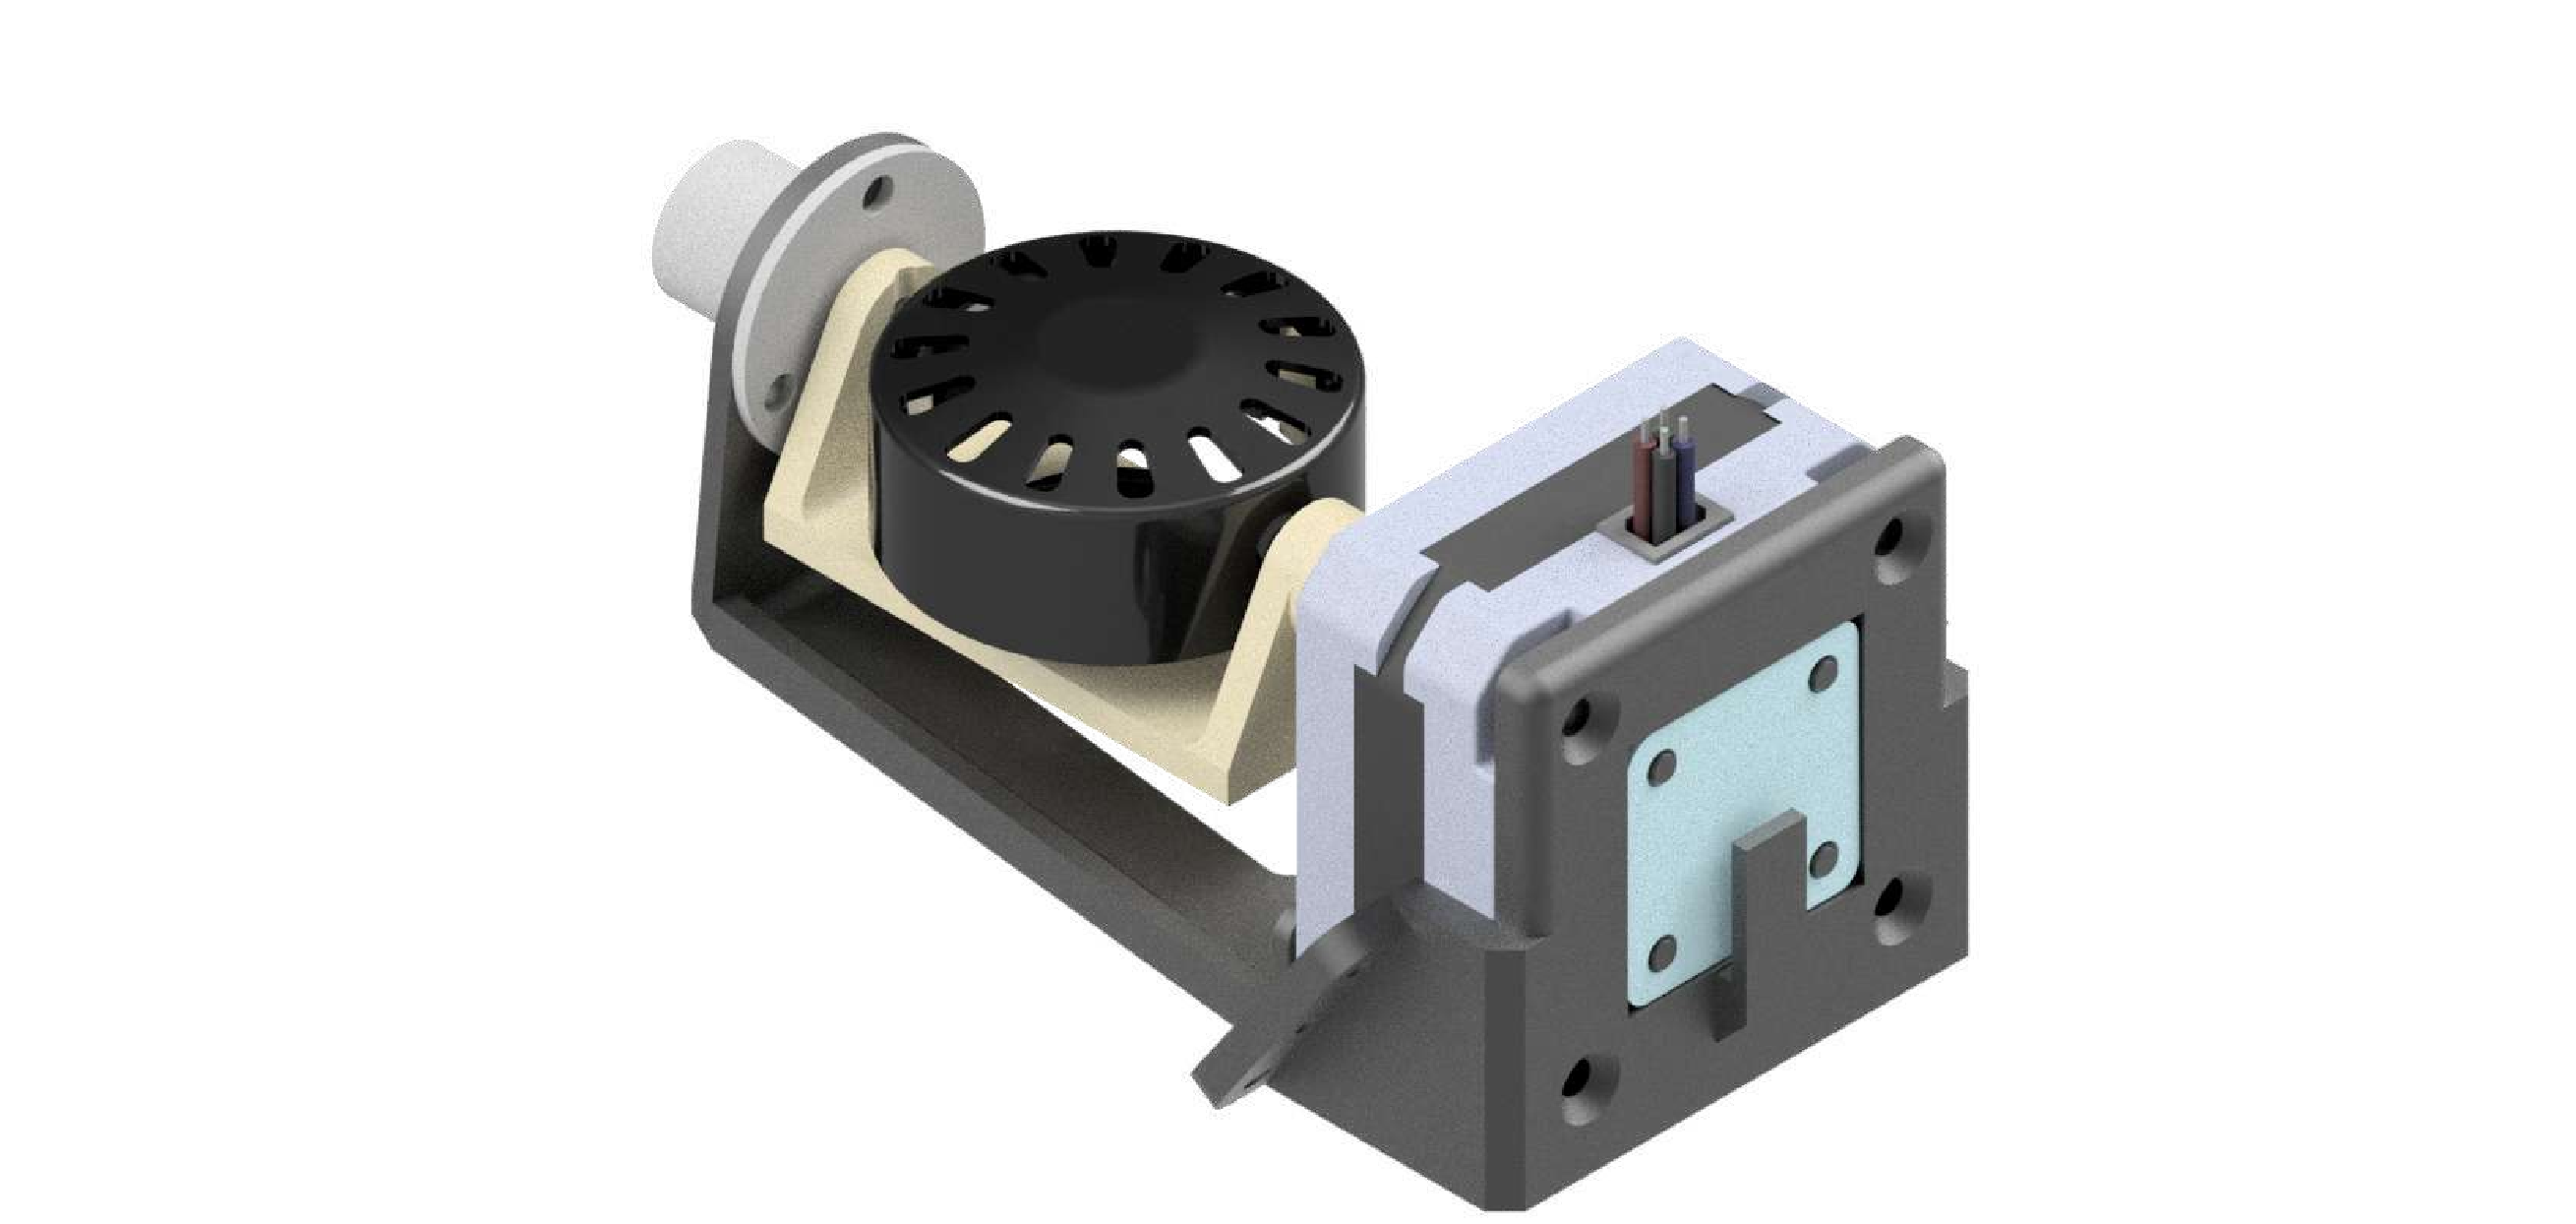
\includegraphics[width=\textwidth]{figures/Assembly/SGCMG.pdf}
    \caption{Sharp tip mounting assembly employed to minimize rotational friction with 360 degree rotational freedom in yaw axis and $\pm 60 \deg$ allowed rotation in roll and pitch axis}
    \label{fig:PLATFORM_TIP_ASM}
\end{figure}
